\bibliography{dissertation}
\appendix

\chapter{AI Usage}
\label{appx:ai_prompt}

I did not directly prompt any Large Language Models, to assist with the writing of my dissertation or implementation. However, as listed in the Supporting Technologies list, I used GitHub Copilot to help with writing some tests for the parser and type checker. I used it via the VS Code extension, which uses the context of your file, to provide advanced AI autocompletion.

I also used AI to transcribe from the audio files of the focus groups (see \ref{appx:additional_mats})

% =============================================================================
\chapter{Additional Materials}
\label{appx:additional_mats}
\begin{figure}[h]
    \centering
    \begin{tabular}{|m{4cm}|p{5cm}|>{\raggedright\arraybackslash}p{5.5cm}|}
        \hline \textbf{File Name} & \textbf{Description} & \textbf{How to Open} \\ \hline
        \verb|Figma_Design.fig| & The Figma Prototype of the design & Using Figma Desktop or Web\\ \hline
        \verb|afg_transcript.pdf| & The AI generated transcript from the audio recording of the advanced focus group & Using a PDF viewer\\ \hline
        \verb|c[2, 3, 4]_end.zip| & The built application as it was at the end of phases 2, 3, 4 respectively & Unzip, and then serve the `list' folder. \newline An easy way is to run \verb|python3 -m http.server 3000| in the `list' folder to serve on port 3000, and then go to \verb|localhost:3000| in the browser. Unfortunately, I was not able to package the end of phase 1 product in a way that was as simple to serve, however \ref{fig:screenshot_phase_1_end} shows what it looked like\\ \hline
    \end{tabular}
\end{figure}


\begin{lstlisting}[language=SFL]
if :: Bool -> a -> a -> a
if cond then_branch else_branch = match cond {
  | true -> then_branch
  | false -> else_branch
}

data Either a b = Left a | Right b
data Maybe a = Just a | Nothing
data List a = Cons a (List a) | Nil

// List Operations
map :: (a -> b) -> List a -> List b
map f list = match list {
  | Nil -> Nil
  | Cons x xs -> Cons (f x) (map f xs)
}

foldr :: (a -> b -> b) -> b -> List a -> b
foldr f acc list = match list {
  | Nil -> acc
  | Cons x xs -> f x (foldr f acc xs)
}

filter :: (a -> Bool) -> List a -> List a
filter pred list = match list :: List a {
  | Nil -> Nil
  | Cons x xs -> if (pred x) (Cons x (filter pred xs)) (filter pred xs)
}

repeat :: a -> List a
repeat n = Cons n $ repeat n

length :: List a -> Int
length xs = foldr (\_ i. i + 1) 0 xs

infiniteFrom :: Int -> List Int
infiniteFrom x = Cons x (infiniteFrom (x + 1))

take :: Int -> List a -> List a
take n list = match list {
  | Nil -> Nil
  | Cons x xs -> if (n > 0) (Cons x (take (n - 1) xs)) (Nil)
}

range :: Int -> Int -> List Int
range lower upper = take (upper - lower) $ infiniteFrom lower

sum :: List Int -> Int
sum = foldr (\x acc. x + acc) 0
\end{lstlisting}

\chapter{Some Example Derivations Using the Type Checking Algorithm}
\label{appx:example_derive}



% \section{Typechecking an Expression Involving Lists}
% We shall attempt to use the algorithm to check the type of $\text{Cons}\;1\;x$ against $Int \fto List\;Int$. This derivation will skip some trivial subtyping/instantiation, but it should serve as a demonstration of how more complex checking works. 

% \begin{mathpar}
% T_{Cons} = \alltype{\alpha}{\alpha \fto List\; \alpha \fto List\;\alpha}\\
% \Gamma_0 = T_{Cons}\and
% \Gamma_1 = \Gamma_0, \ahat, \bhat, x : \ahat \\

% \Infer{\Sub[1]}
%     {
%         [2]
%         \\
%         \subjudg{\Theta}{[\Theta]A}{[\Theta]B}{\Delta}
%     }
%     {\chkjudg{\Gamma}{\lam{x} Cons\;1\;x}{List\;Int}{\Delta}}

% \\

% {\Infer{{\!\ArrIntroSyn}[2]}
%     {
%     \chkjudg{\Gamma_1}{Cons\;1\;x}{\bhat}{\Delta, x : \ahat, \Theta}
%     }
%     {{\synjudg{\Gamma_0}{\lam{x} Cons\;1\;x}{\ahat \arr \bhat}{\Delta}}}

%     \Infer{\!\ArrElim[3]}
%         {
%         {
%             [4]{\synjudg{\Gamma_1}{Cons\,1}{C}{\Delta}}
%         }
%         \\
%         \appjudg{\Gamma_1}{x}{[\Gamma_1]A}{C}{\Delta}
%         }
%         {\synjudg{\Gamma}{Cons\,1\,x}{C}{\Delta}}
% }

% \\
% \Infer{\!\ArrElim[4]}
%     {
%     {
%     \Infer{\Var}
%         {(Cons : T_{Cons}) \in \Gamma_1}
%         {\synjudg{\Gamma_1}{Cons}{T_{Cons}}{\Gamma_1}}
%     }
%     \\
%     {
%      \Infer{\AllApp}
%         {\appjudg{\Gamma_1,\ahat}{1}{(\ahat \fto List\; \ahat \fto List\;\ahat)}{C}{\Delta}}
%         {\appjudg{\Gamma_1}{1}{\alltype{\alpha}{\alpha \fto List\; \alpha \fto List\;\alpha}}{C}{\Delta}}
%     }
%     }
%     {\synjudg{\Gamma_1}{Cons\,1}{C}{\Delta}}
% \end{mathpar}


\section{Typechecking an Expression Involving Lists}
We shall attempt to use the algorithm to check the type of $\text{Cons}\;1\;x$ against $List\;Int$. This derivation should serve as a demonstration of how more complex checking works. This derivation assumes $Cons$ and $Nil$ are defined over $Int$s only. The reason the context is never changed is as we do not have any abstractions or foralls, so no variables or type variables are introduced.

\begin{mathpar}
T_{Nil} = List\;Int\and
T_{Cons} = {Int \fto List\;Int \fto List\;Int}\\
\Gamma = T_{Cons}, T_{Nil}\and\Gamma = \Gamma_0 = \Gamma_1\\

\\

\Infer{\MyTCRule{\Unionsubrulename}[10]}
    {\Infer{\MyTCRule{\Intsubrulename}[11]}{ }
        {\subjudg{\Gamma_0}{\Inttype}{\Inttype}{\Gamma_1}}}
    {\subjudg{\Gamma_0}{List[Int]}{List[Int]}{\Gamma_{1}}}
\\

\Infer{\ArrApp[7]}
    {     \Infer{\Sub[8]}
          { 
          {
          \Infer{\Var[9]}
            {(Nil : T_{Nil}) \in \Gamma}
            {\synjudg{\Gamma}{Nil}{T_{Nil}}{\Gamma}}
          }
            \\
            [10]\subjudg{\Gamma}{List[Int]}{List[Int]}{\Gamma}
          }
          {\chkjudg{\Gamma}{Nil}{List\;Int}{\Gamma}}}
    {\appjudg{\Gamma}{Nil}{List\;Int \arr List\;Int}{List\;Int}{\Gamma}}

\\
\Infer{\!\ArrElim[3]}
{
{
\Infer{\Var[4]}
    {(Cons : T_{Cons}) \in \Gamma}
    {\synjudg{\Gamma}{Cons}{T_{Cons}}{\Gamma}}
}
\\
    {
    \Infer{\ArrApp[5]}
        {
        \Infer{\MyTCRule{\Intcheckrulename}[6]}
            { }
            {\chkjudg{\Gamma}{1}{\Inttype}{\Gamma}}
        }
        {\appjudg{\Gamma}{1}{T_{Cons}}{List\;Int \arr List\;Int}{\Gamma}}
     % \Infer{\AllApp}
     %    {\appjudg{\Gamma_1,\ahat}{1}{(\ahat \fto List\; \ahat \fto List\;\ahat)}{C}{\Delta}}
     %    {\appjudg{\Gamma_1}{1}{\alltype{\alpha}{\alpha \fto List\; \alpha \fto List\;\alpha}}{C}{\Delta}}
    }
    }
    {\synjudg{\Gamma}{Cons\,1}{List\;Int \arr List\;Int}{\Gamma}}
\\

\Infer{\!\ArrElim[2]}
    {
    {
        [3]{\synjudg{\Gamma}{Cons\,1}{List\;Int \arr List\;Int}{\Gamma}}
    }
    \\
    [7]\appjudg{\Gamma}{Nil}{List\;Int \arr List\;Int}{List\;Int}{\Gamma}
    }
    {\synjudg{\Gamma}{Cons\,1\,Nil}{List\;Int}{\Gamma}}
\\

\Infer{\Sub[1]}
    {
        [2]{\synjudg{\Gamma}{Cons\,1\,Nil}{List\;Int}{\Gamma}}
        \\
        [10]\subjudg{\Gamma}{List[Int]}{List[Int]}{\Gamma}
    }
    {\chkjudg{\Gamma}{Cons\;1\;Nil}{List\;Int}{\Gamma}}
\end{mathpar}

\begin{enumerate}
    \item To check $Cons\;1\;Nil$ against $List\;Int$ [2], we first synthesise the expression type, and check the synthesised type is as subtype of $List\;Int$ [10].
    \item To synthesise the type of the expression $Cons\;1\;Nil$ (implicitly $((Cons\;1)\;Nil)$) we synthesise the type of the left hand side of the application $Cons\;1$ to be $List\;Int\arr List\;Int$ [7] and then we synthesise the type of $Nil$ under the application of that type, which gives us $List\;Int$.
    \item To synthesise the type of $Cons\;1$, we synthesise the type of the left hand side of the application $Cons$ to be $T_{Cons}: Int\arr List\;Int\arr List\;Int$ [4], and then synthesise the type of $1$ under the application of that type, which gives us $List\;Int\arr List\;Int$ [5].
    \item We synthesise the type of $Cons$ to be $T_{Cons}$ from the context.
    \item We synthesise the type of $1$ under the application of $T_{Cons}$, by first checking the type of $1$ against the type $Int$ which is the left hand side of the applied type[6]. This allows us to synthesise the right hand side of the applied type: $List\;Int\arr List\;Int$. 
    \item 1 checks against the type $Int$, as it is an Int literal.
    \item To synthesise the type of $Nil$ under the application of $List\;Int\arr List\;Int$, we check $Nil$ against the type $List\;Int$ which is the left hand side of the applied type[8]. This allows us to synthesise the right hand side of the applied type: $List\;Int$
    \item To check $Nil$ against the type $List\;Int$, we first synthesise the type of $Nil$ resulting in $T_{Nil} :List\;Int$[9]. We then check that this is a subtype of $List\;Int$[10].
    \item We synthesise the type of $Nil$ to be $T_{Nil}$ from the context.
    \item We apply the \MyTCRule{\Unionsubrulename} rule to check that $List\;Int$ is a subtype (non strict) of $List\;Int$. The first check is that the names are the same, as the names uniquely identify these types. We then iterate over the list of the arguments to the type constructor. The name of the context increments to reflect this iteration, but the context is unchanged during this check. There is only one type in the list
\end{enumerate}

\chapter{Pattern Matching Algorithm}
A pattern consists of only:
\begin{itemize}
    \item An application
    \item A literal
    \item A pair
    \item An identifier: could be a wildcard, a constructor.
\end{itemize}

Below is the algorithm for each of these cases, as well as the top level pattern matching algorithm. 

\begin{figure}[h]
    \begin{lstlisting}[language=Rust_boxed]
fn get_redex_from_match(match_expression) -> Option<RedexContractionPair> {
    // get the expression being matched
    let expr = match_expression.to_be_matched
    // Iterate through all the patterns and their resulting expressions
    for ((pattern, resulting_expr) in match_expression.cases) {
        let result = pattern_match(expr, pattern);
        if (result == Refute) {
            // If refuted, then we can safely consider next pattern
            continue
        }
        if (result == Unknown) {
            // We get the reduction option for the expression
            // as we cannot refute this pattern
            return get_redex(expr)
        }
        if (result == Success(bindings)) {
            return Some(RedexContractionPair {
                from: match_expression,
                to: resulting_expr.substitute(bindings),
                reduction_message: "Match to pattern" + pattern.to_string()
            })
        }
    }
    // Refuted all patterns
    return None
}
\end{lstlisting}
    \caption{The algorithm for getting the redex-contraction pair from a match expression. If we sucessfully match, the result will be the expression corresponding to the matching pattern. If we cannot match expressions}
    \label{fig:all_pattern_list_iterate}
\end{figure}

\begin{figure}[h]
    \begin{lstlisting}[language=Rust_boxed]
fn pattern_match(expr, pattern) -> MatchResult {
    if (pattern is identifier) {match_against_identifier(expr, pattern)}
    if (pattern is a pair) {match_against_pair(expr, pattern)}
    if (pattern is an app) {match_against_application(expr, pattern)}
    if (pattern is a literal) {
        if (expr.to_string() == pattern.to_string()) 
            return Success([])
        } else {
            return Refute
        }
    }
}
\end{lstlisting}
    \caption{The algorithm for matching an expression against a pattern}
    \label{fig:pattern_list_top_level}
\end{figure}

\begin{figure}[h]
    \begin{lstlisting}[language=Rust_boxed]
fn match_against_identifier(expr, pattern) -> MatchResult {
    if (pattern is "_") {
        // Succeed but dont bind anything
        Success([])
    }
    if (pattern is a lowercase identifier) {
        // We suceed as a lowercase ID is a wildcard, and we must add to 
        // our list of bindings the fact that the named wildcard now has a 
        // value: the expr
        Success([(pattern.string, expr)])
    }
    if (pattern is a constructor (i.e. is uppercase)) {
        if (expr is also a constructor with the same name) {
            return Success([])
        }
        if (expr is an application) {
            // `Head' refers to the recursive front of an application. For 
            // instance, The head of (Left ((Cons x) xs)) would be Left.
            if (the head of expr is a constructor) {
                // We can refute, as constructors never evaluate, so the 
                // structure of the expression will never be the same as
                // the pattern. 
                return Refute
            } else {
                // Otherwise further evaluation might lead to a pattern 
                // that matches this constructor so we cant refute yet
                return Unknown
            }
        }
        return Unknown;
    }
}
    \end{lstlisting}
    \caption{The algorithm for matching an expression against a pattern that is an identifier in rust like pseudocode}
    \label{fig:pattern_list_id}
\end{figure}

\begin{figure}[h]
    \begin{lstlisting}[language=Rust_boxed]
fn match_against_pair(expr, pattern) -> MatchResult {
    if (expr is also a pair) {
        let first = pattern_match(expr.first, pattern.first);
        let second = pattern_match(expr.second, pattern.second);

        // Propogate refute and unknown
        if (first == Unknown || second == Unknown) {
            return Unknown;
        }
        if (first == Refute || second == Refute) {
            return Refute;
        }
        // first and second have suceeded, return both sets of bindings
        return Success(first.bindings + second.bindings)
    }
    if (expr is an application) {
        if (the head of expr is a constructor) {
            return Refute
        } else {
            return Unknown
        }
    }
    if (expr is a literal || expr is an abstraction) {return Refute}    
    
    return Unknown // catchall: only `match'
}
\end{lstlisting}
    \caption{The algorithm for matching an expression against a pattern that is a pair in rust like pseudocode. See \ref{fig:pattern_list_id} for more detail about the `expr is application' case}
    \label{fig:pattern_list_pair}
\end{figure}

\begin{figure}[h]
    \begin{lstlisting}[language=Rust_boxed]
fn match_against_application(expr, pattern) -> MatchResult {
    if (expr is also an application) {
        let func = pattern_match(expr.func, pattern.func);
        let arg = pattern_match(expr.arg, pattern.arg);

        // Propogate refute and unknown
        if (func == Unknown || arg == Unknown) {
            return Unknown;
        }
        if (func == Refute || arg == Refute) {
            return Refute;
        }
        // func and arg have suceeded, return both sets of bindings
        return Success(func.bindings + arg.bindings)
    }
    if (expr is a literal || expr is a pair 
        || expr is an abstraction) {return Refute}
    return Unknown
}
\end{lstlisting}
    \caption{The algorithm for matching an expression against a pattern that is a pair in rust like pseudocode. See \ref{fig:pattern_list_id} for more detail about the `expr is application' case}
    \label{fig:pattern_list_app}
\end{figure}


\begin{figure}[t]
    \begin{tabular}{c}
    \begin{lstlisting}[language=Rust_boxed]
enum DiffElem {
    Similarity(String), 
    Difference(String, String)
}
type Diff = Vec<DiffElem>
// rust-like psuedocode, not valid rust
// ast1 and 2 are the two ASTs, and expr1 and 2 are the indices
// of the terms we are considering for our diff. 
fn diff(ast1, ast2, expr1, expr2) -> Diff {
    node1, node2 = ast1.get(expr1), ast2.get(expr2)
    diff = Diff::new();
    match (node1, node2) {
        // IDs and Lits are compared based on their string "values"
        (ID, ID) |
        (Lit, Lit) => {
            if node1.value == node2.value {
                diff += Similarity(node1.value)
            } else {
                diff += Difference(node1.value, node2.value)
            }
        }
        (Pair {first1, second1}, Pair {first2, second2}) => {
            // As both are pairs, their opening brackets, 
            // commas, and closing brackets are in common.
            // We get the diff of the first and second
            // element to find the diff of the whole pair 
            diff += Similarity("(")
            diff += diff(ast1, ast2, first1, first2)
            diff += Similarity(",")
            diff += diff(ast1, ast2, second1, second2)
            diff += Similarity(")")
        }
        ...
    }
    return diff;
}
    \end{lstlisting}
    \end{tabular}
    \caption{rust-like psuedocode listing for the type of the output of the diff function, as well as a small section of the algorithm. There is also (not shown) a wrapper around the Diff type, to allow for conversion into JavaScript (see \ref{bg:wasm}), as well as the some logic for combining diffs.}
    \label{fig:diff_list}
\end{figure}

\chapter{Tokens for Lexical Analysis}
\label{appx:tokens}
Below is the code for how tokens outputted by lexical analysis are defined. 
\begin{lstlisting}
enum TokenType {
    EOF,
    Newline,

    Id,
    UppercaseId,

    If,
    Then,
    Else,

    Match,
    LBrace,
    RBrace,

    IntLit,
    FloatLit,
    StringLit,
    CharLit,
    BoolLit,

    DoubleColon,
    RArrow,
    Forall,
    KWType,
    KWData,

    LParen,
    RParen,

    Lambda,

    Dollar,
    Dot,
    Comma,
    Bar,

    Assignment,
}

struct Token {
    tt: TokenType,
    value: String,
}
\end{lstlisting}

\chapter{UI Screenshots}
\begin{figure}[h]
    \centering
    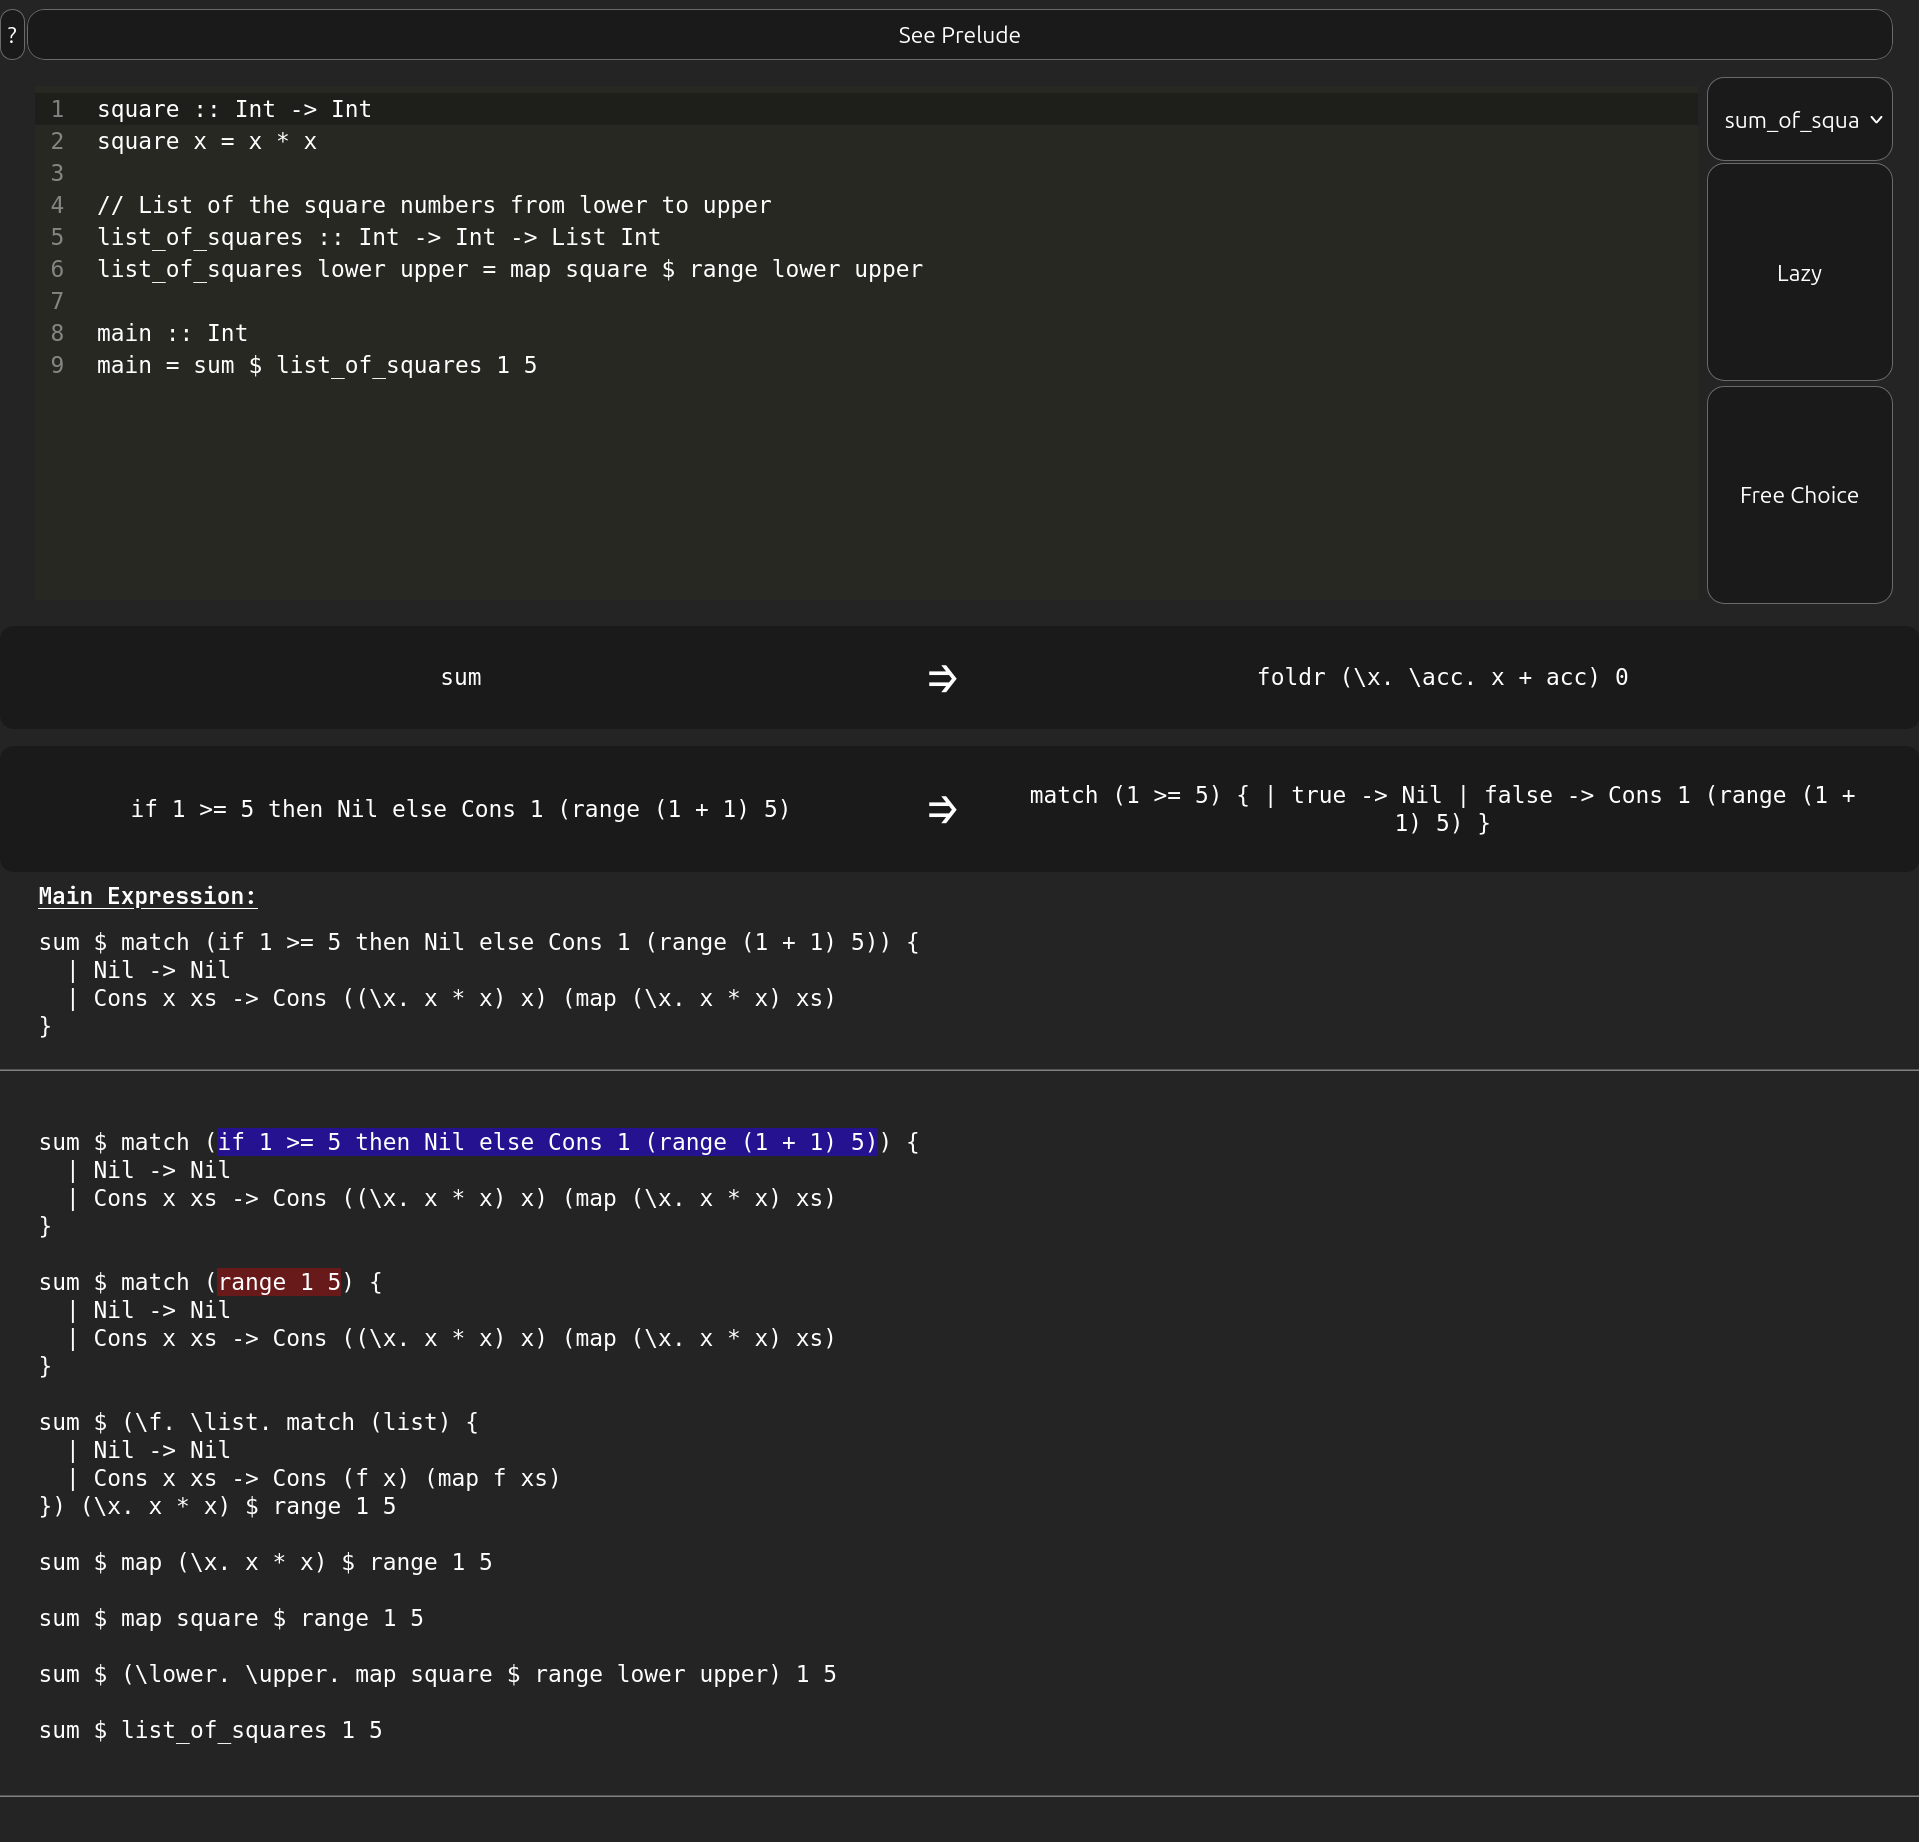
\includegraphics[width=1\linewidth]{images/phase-2-end3.png} 
    \captionsetup{justification=centering}
    \caption{The product at the end of phase two during free choice evaluation of the `sum of squares' sample program, with the prelude dropdown contracted}
    \label{fig:screenshot_c2_end_free}
\end{figure}

\begin{figure}[h]
    \centering
    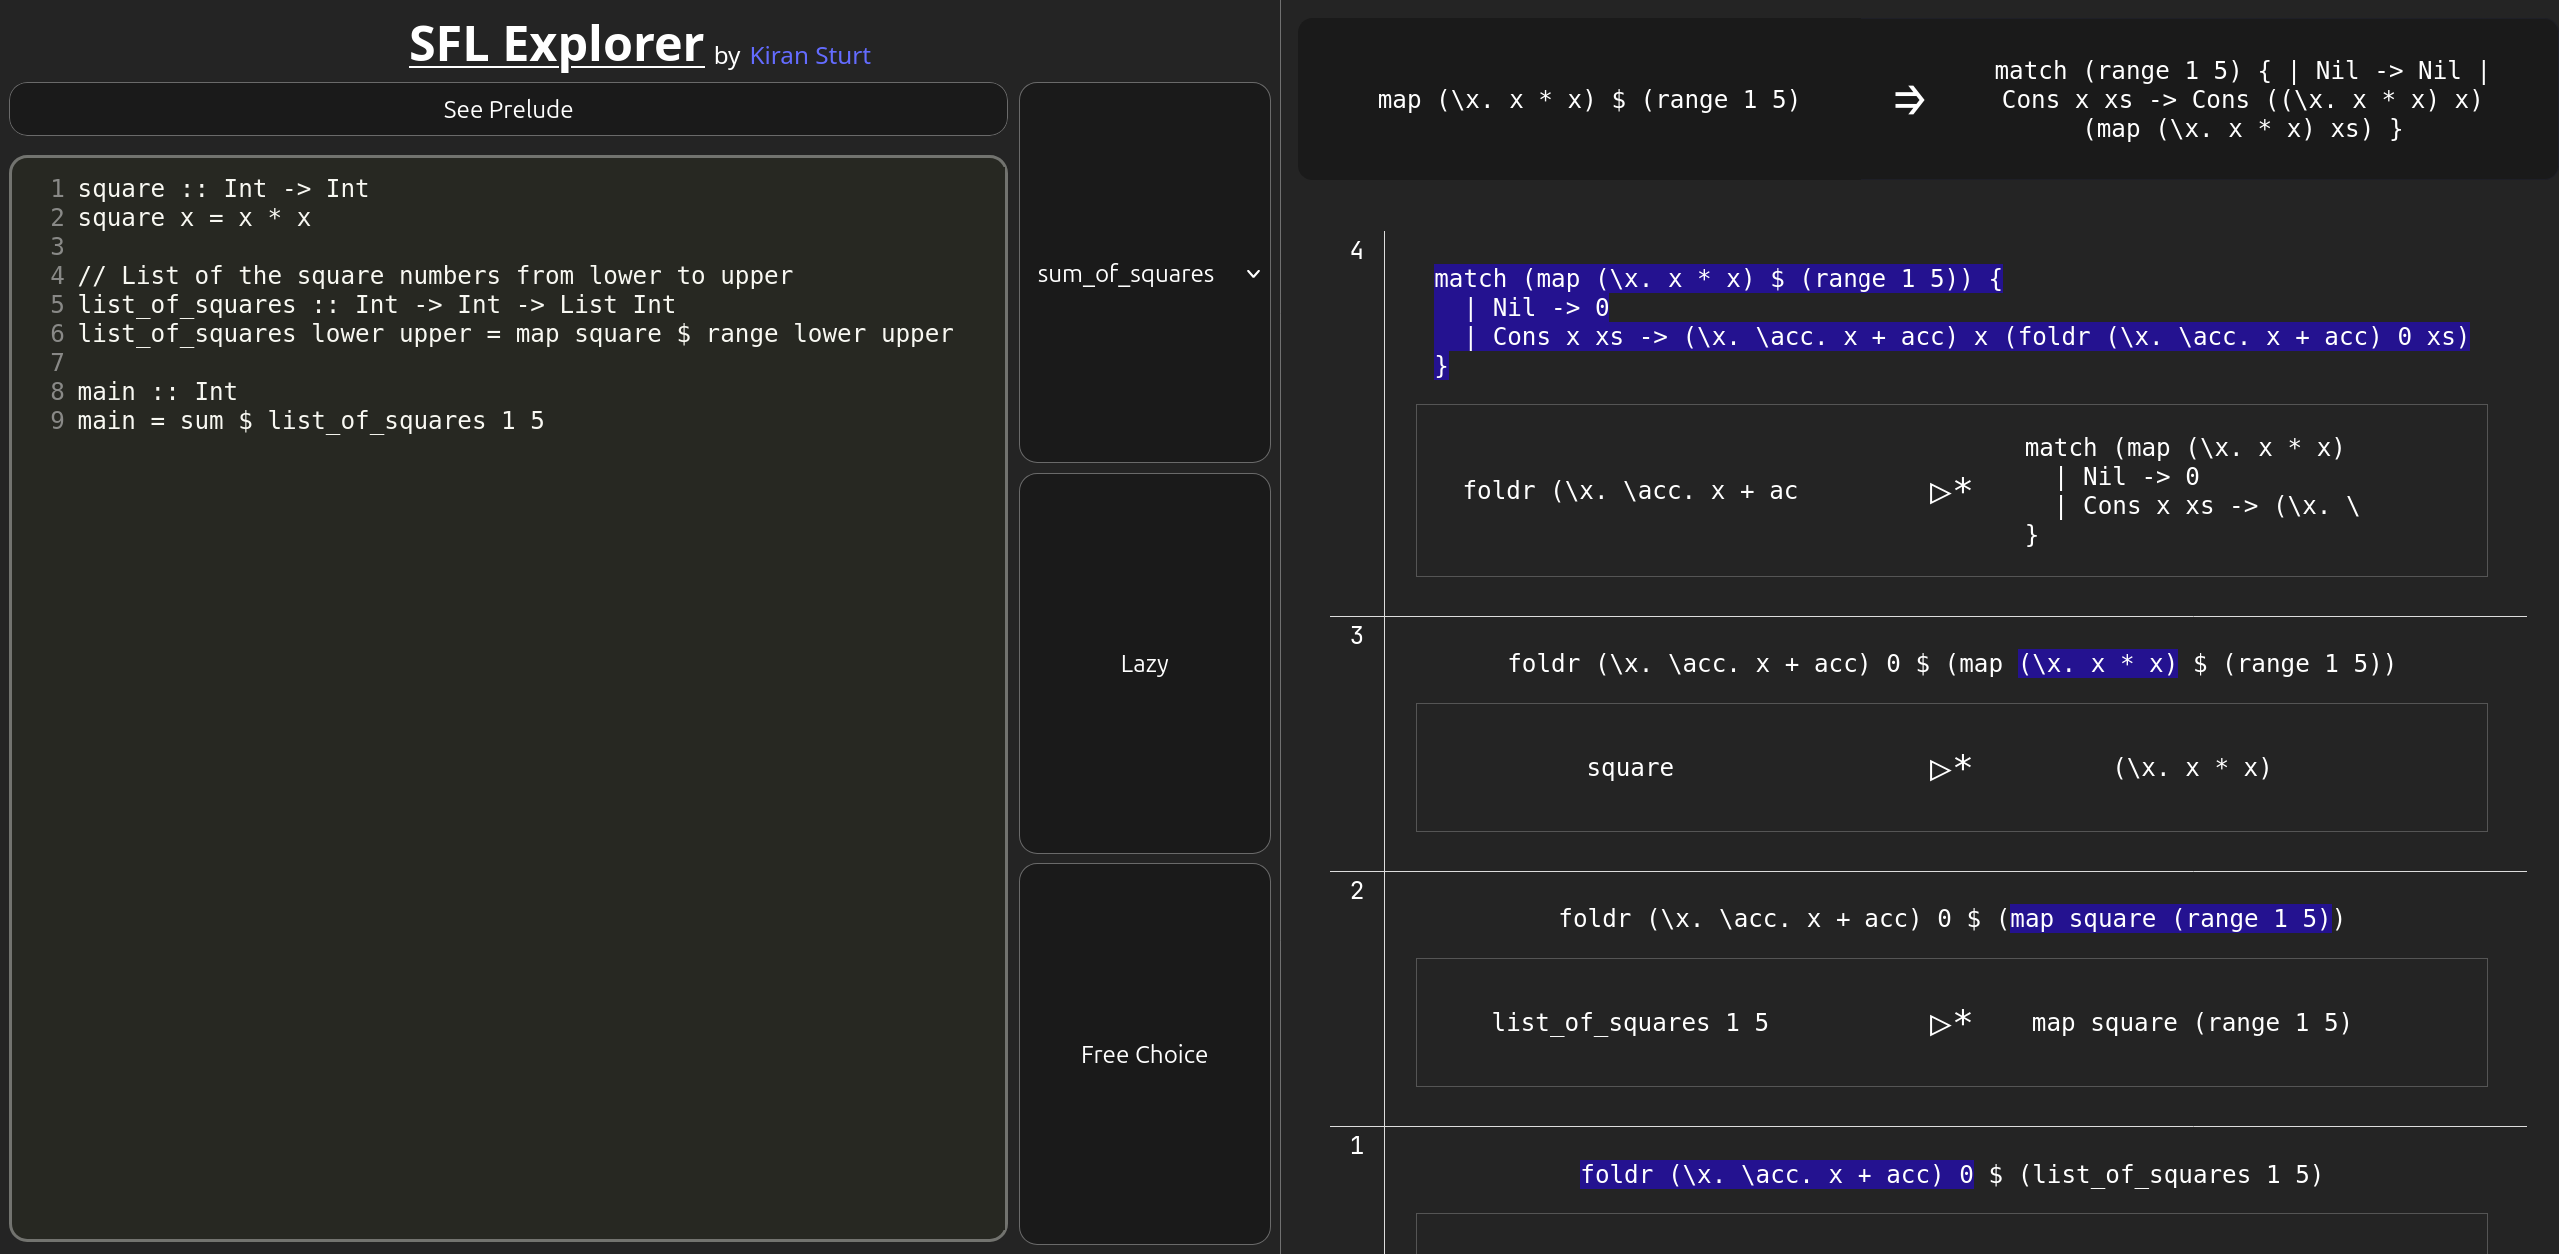
\includegraphics[width=\linewidth]{images/phase-3-end-free.png}
    \caption{The new UI implemented at the end of phase three, during free choice evaluation of the provided `sum of squares' example program}
    \label{screenshot:phase3_end_free}
\end{figure}

\begin{figure}[h]
    \centering
    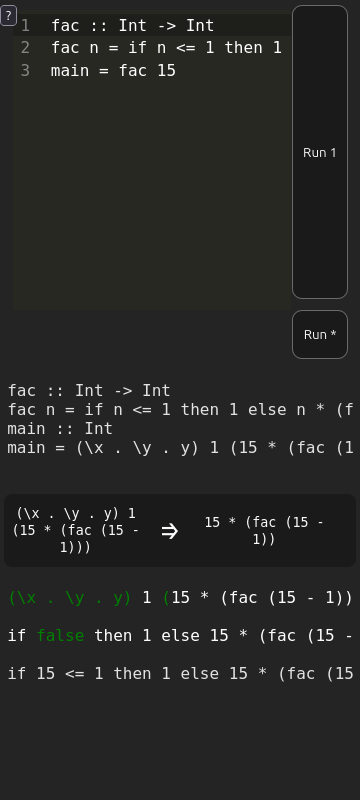
\includegraphics[width=0.3\linewidth]{images/testathon-mobile.png}
    \caption{The UI as it appeared at the end of phase 2, as it would have appeared on a Samsung Galaxy S20}
    \label{fig:screenshot_phase2_mobile}
\end{figure}

\begin{figure}[h]
    \centering
    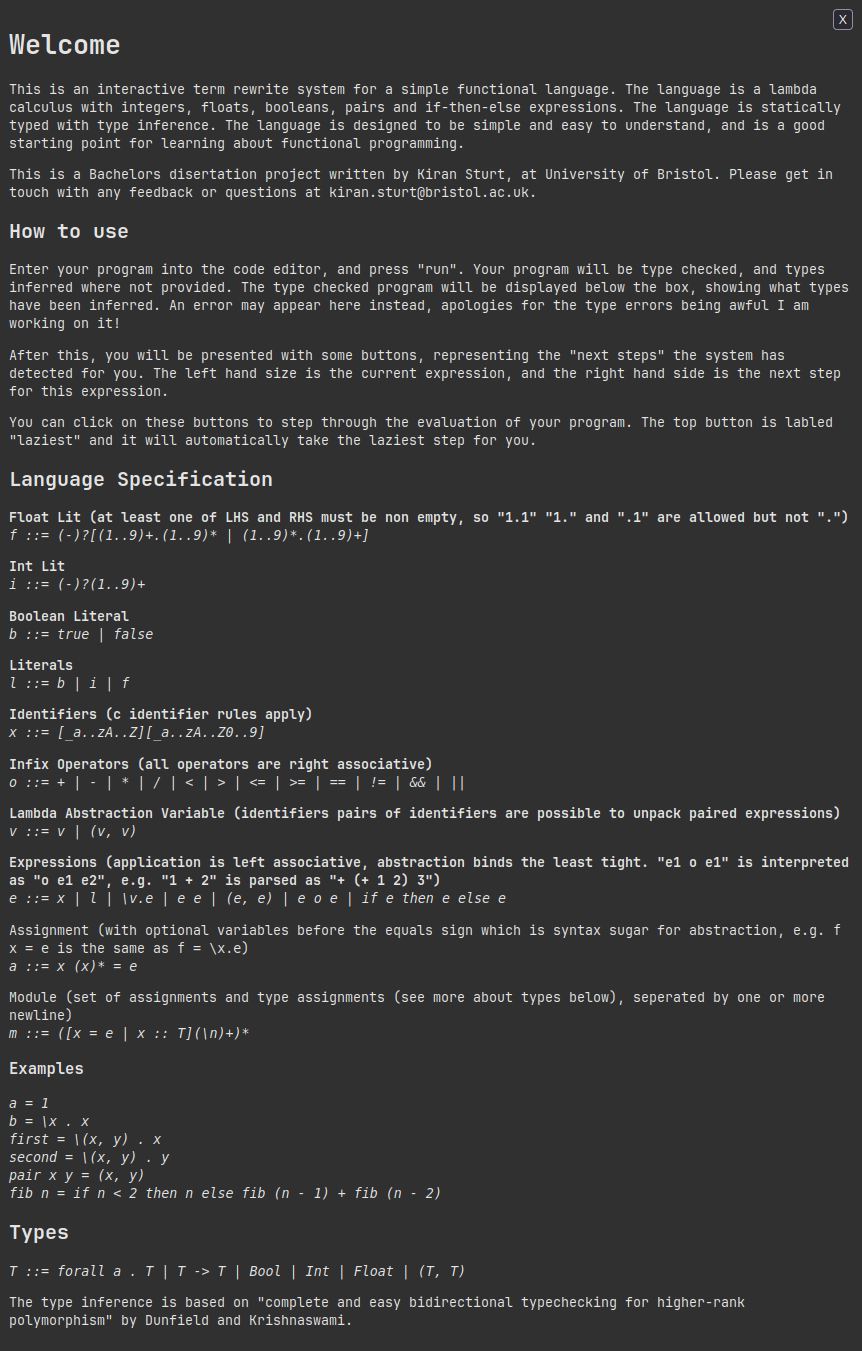
\includegraphics[width=0.9\linewidth]{images/testathon_help_menu_cropped.png} 
    \captionsetup{justification=centering}
    \caption{The `Help menu' in the proof of concept UI. This was spawned by pressing the `?' button in the top left of the UI, and dismissed by pressing the `X' button, or clicking outside the box}
    \label{fig:screenshot_phase2_help}
\end{figure}

\begin{figure}[h]
    \centering
    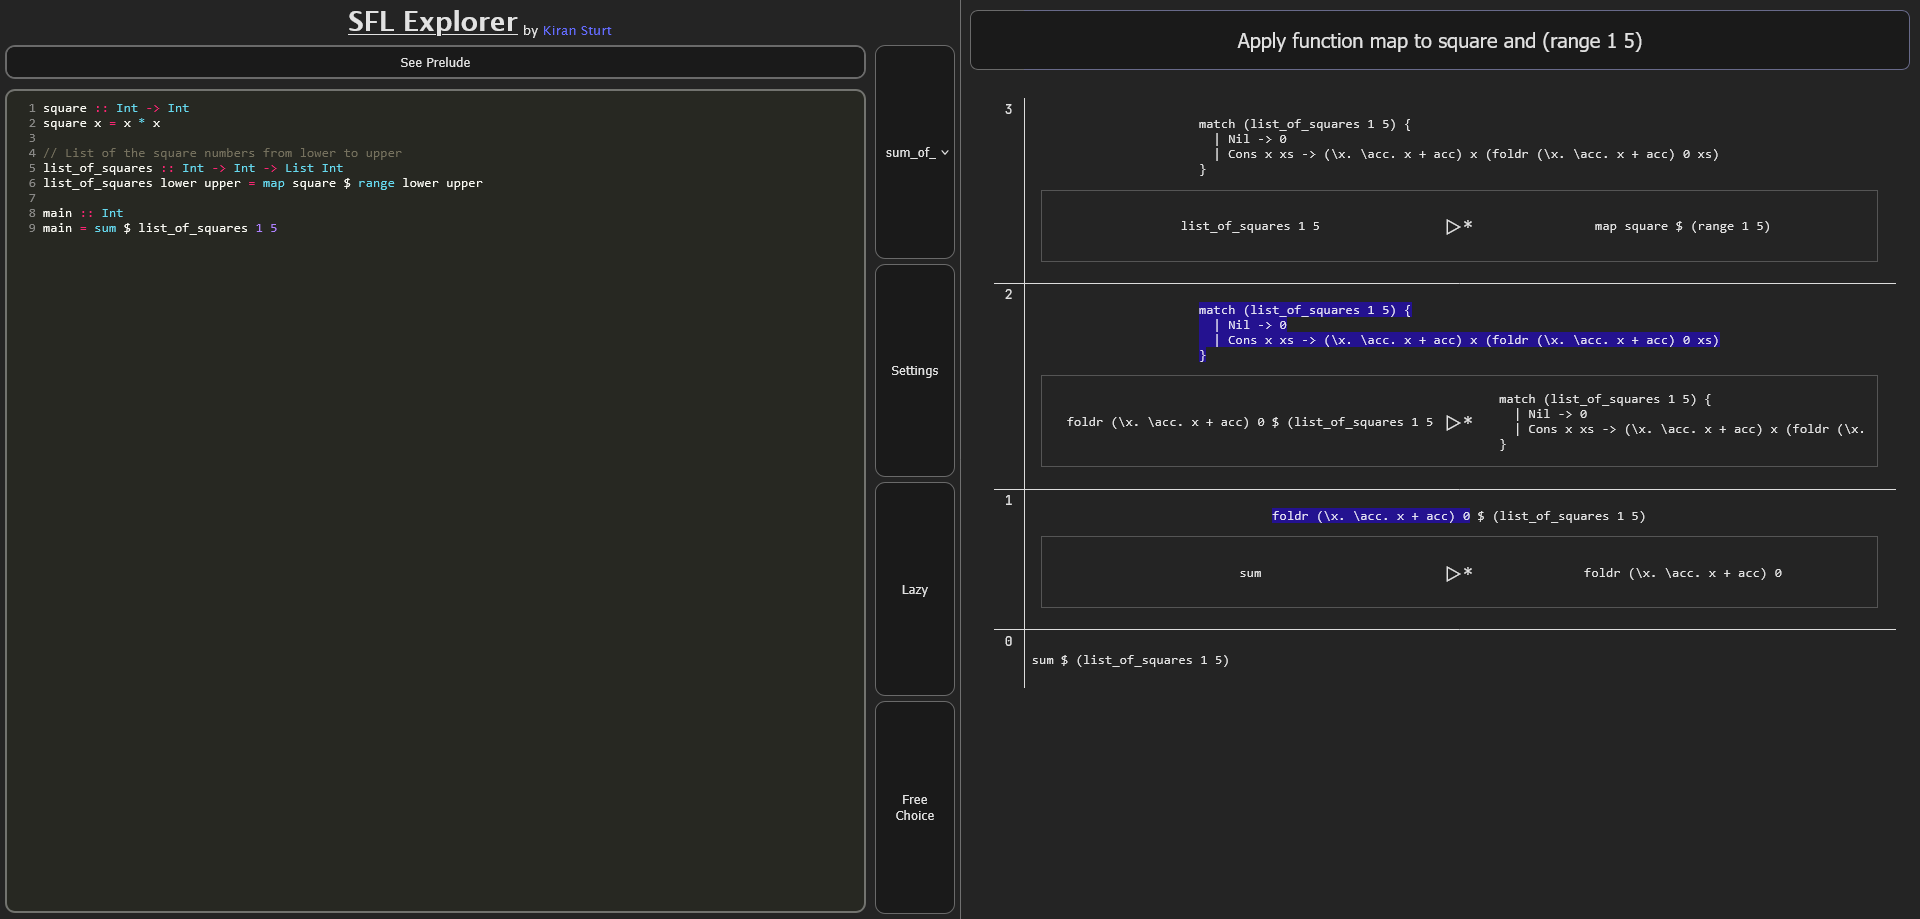
\includegraphics[width=\linewidth]{images/final_dark.png} 
    \captionsetup{justification=centering}
    \caption{The final product during lazy evaluation of the `sum of squares' sample program}
    \label{fig:screenshot_final_dark}
\end{figure}

\begin{figure}[h]
    \centering
    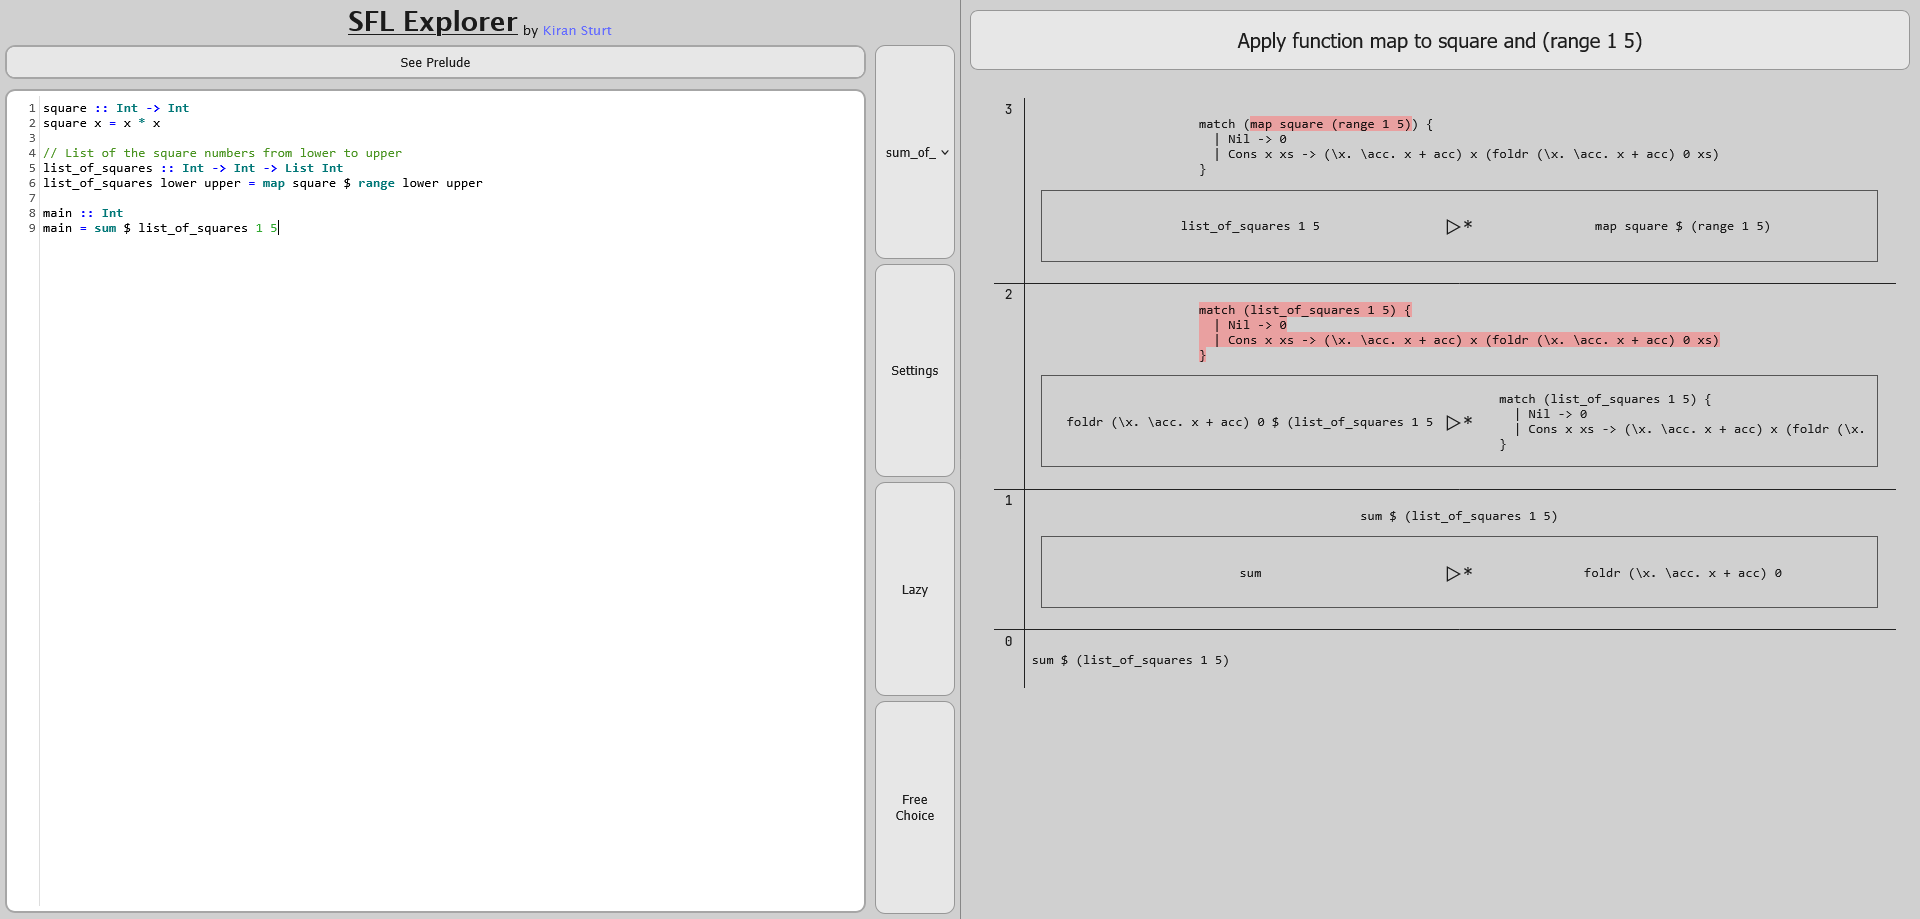
\includegraphics[width=\linewidth]{images/final_light.png} 
    \captionsetup{justification=centering}
    \caption{The final product during lazy evaluation of the `sum of squares' sample program in light mode}
    \label{fig:screenshot_final_light}
\end{figure}

\begin{figure}[h]
    \centering
    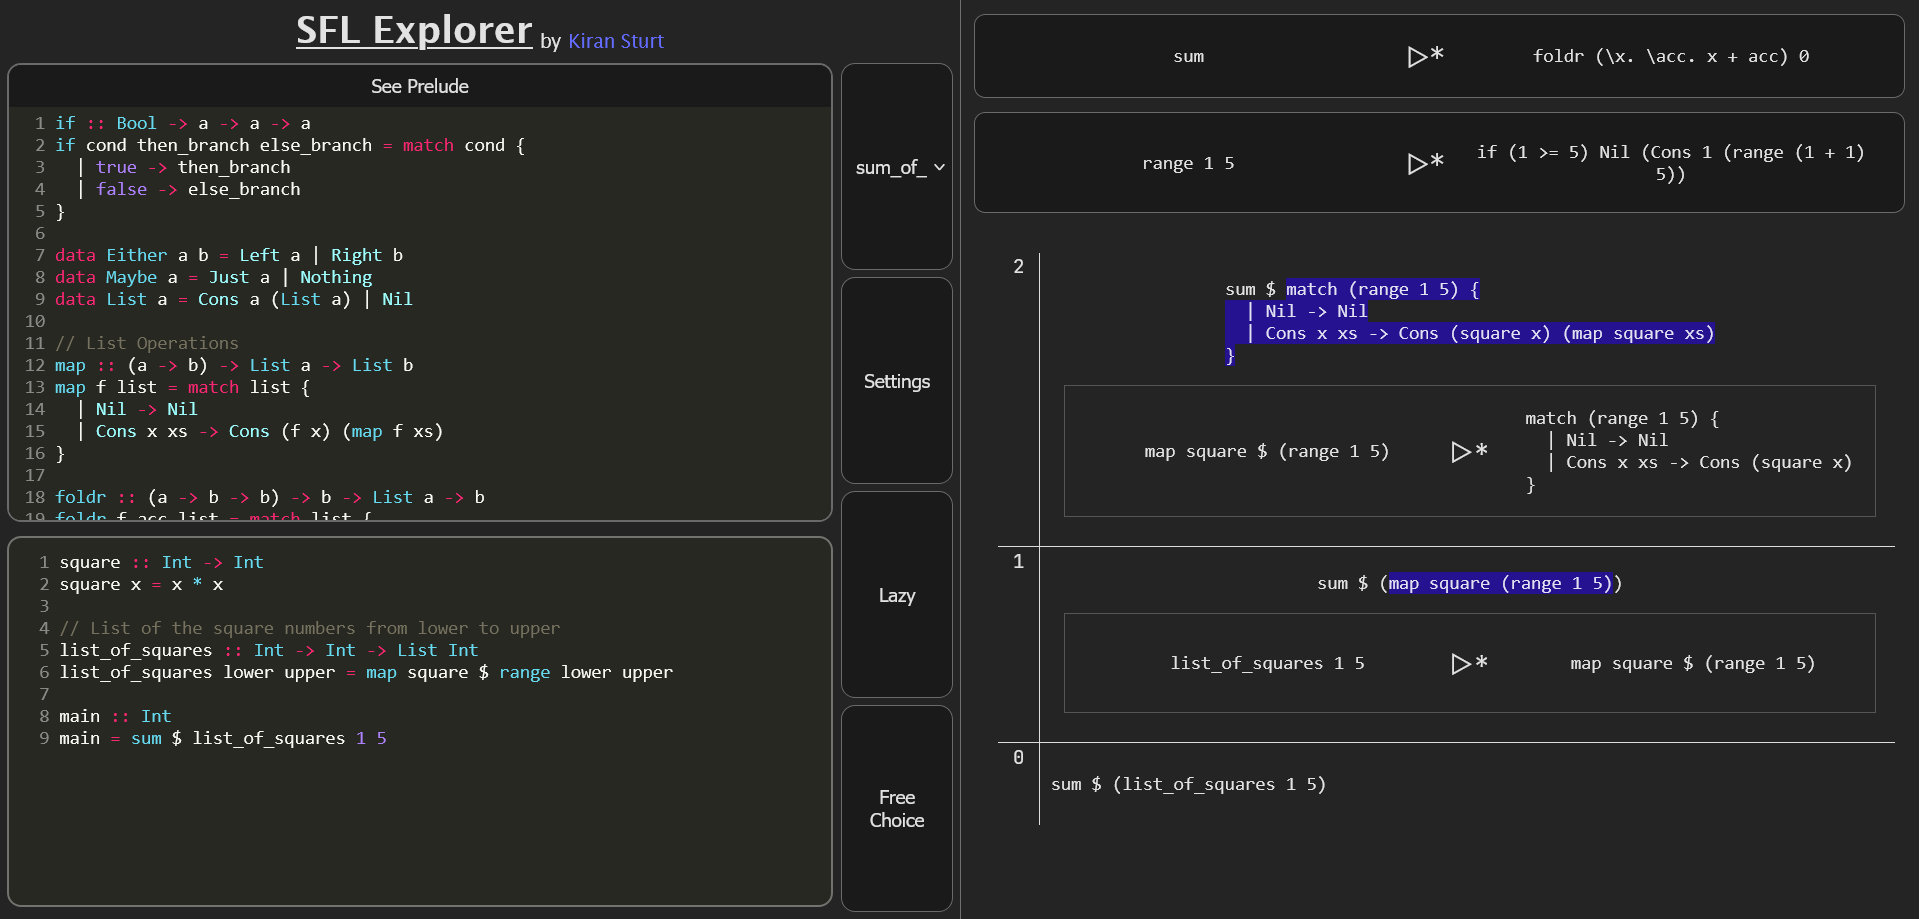
\includegraphics[width=\linewidth]{images/final_dark_prelude_free.png} 
    \captionsetup{justification=centering}
    \caption{The final product during free choice evaluation of the `sum of squares' sample program, with the prelude visible}
    \label{fig:screenshot_final_dark_prelude_free}
\end{figure}

\begin{figure}[h]
    \centering
    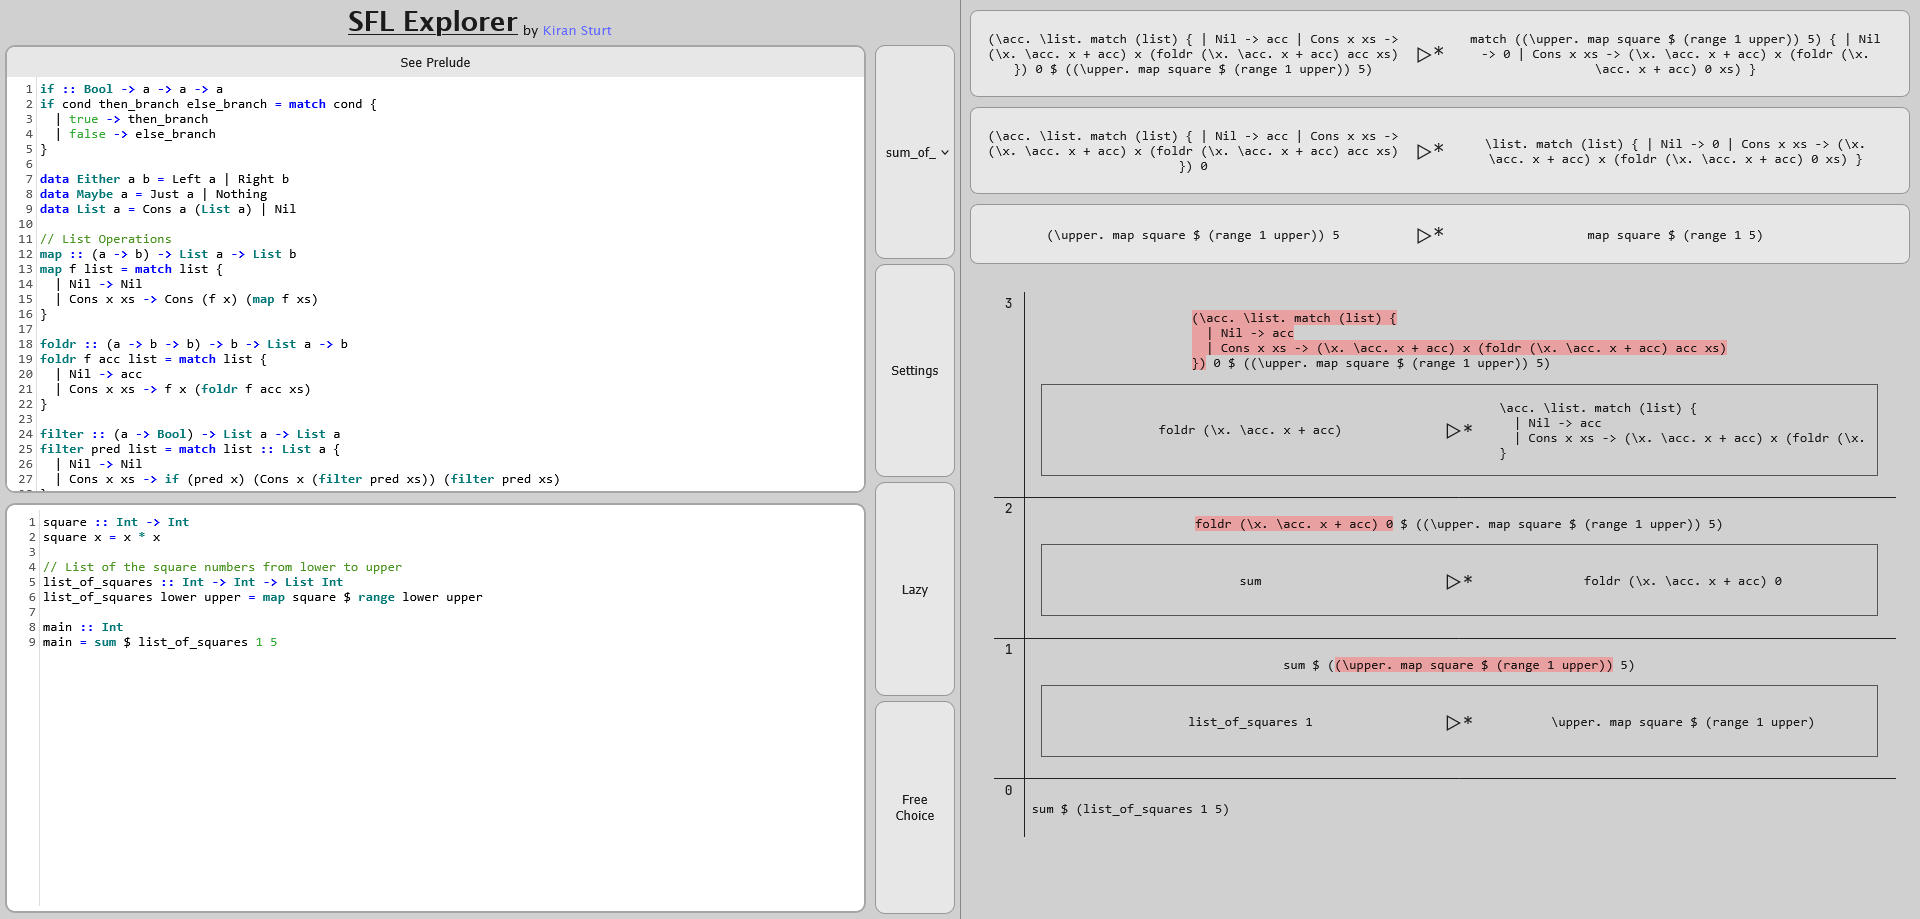
\includegraphics[width=\linewidth]{images/final_light_prelude_free.png} 
    \captionsetup{justification=centering}
    \caption{The final product during free choice evaluation of the `sum of squares' sample program, with the prelude visible in light mode}    
    \label{fig:screenshot_final_light_prelude_free}
\end{figure}

% \chapter{Language Grammar}
% \input{sections/lang_grammar}

